\documentclass{book}
\usepackage[a4paper,top=2.5cm,bottom=2.5cm,left=2.5cm,right=2.5cm]{geometry}
\usepackage{makeidx}
\usepackage{natbib}
\usepackage{graphicx}
\usepackage{multicol}
\usepackage{float}
\usepackage{listings}
\usepackage{color}
\usepackage{ifthen}
\usepackage[table]{xcolor}
\usepackage{textcomp}
\usepackage{alltt}
\usepackage[utf8]{inputenc}
\usepackage{mathptmx}
\usepackage[scaled=.90]{helvet}
\usepackage{courier}
\usepackage{sectsty}
\usepackage[titles]{tocloft}
\usepackage{doxygen}
\lstset{language=C++,inputencoding=utf8,basicstyle=\footnotesize,breaklines=true,breakatwhitespace=true,tabsize=8,numbers=left }
\makeindex
\setcounter{tocdepth}{3}
\renewcommand{\footrulewidth}{0.4pt}
\renewcommand{\familydefault}{\sfdefault}
\hfuzz=15pt
\setlength{\emergencystretch}{15pt}
\hbadness=750
\tolerance=750
\begin{document}
\begin{titlepage}
\vspace*{7cm}
\begin{center}
{\Large Phil\-Robokit Coding Guidelines }\\
\vspace*{1cm}
{\large Generated by Doxygen 1.8.1.1}\\
\vspace*{0.5cm}
{\small Sat Jul 14 2012 16:19:15}\\
\end{center}
\end{titlepage}
\clearemptydoublepage
\pagenumbering{roman}
\tableofcontents
\clearemptydoublepage
\pagenumbering{arabic}
\chapter{File Index}
\section{File List}
Here is a list of all files with brief descriptions\-:\begin{DoxyCompactList}
\item\contentsline{section}{{\bf Analog\-Output.\-phr} }{\pageref{_analog_output_8phr}}{}
\item\contentsline{section}{{\bf Blink\-Without\-Delay.\-phr} }{\pageref{_blink_without_delay_8phr}}{}
\item\contentsline{section}{{\bf corelib\-\_\-8bit\-\_\-timer.\-c} }{\pageref{corelib__8bit__timer_8c}}{}
\item\contentsline{section}{{\bf corelib\-\_\-8bit\-\_\-timer.\-h} }{\pageref{corelib__8bit__timer_8h}}{}
\item\contentsline{section}{{\bf corelib\-\_\-adc.\-c} }{\pageref{corelib__adc_8c}}{}
\item\contentsline{section}{{\bf corelib\-\_\-adc.\-h} }{\pageref{corelib__adc_8h}}{}
\item\contentsline{section}{{\bf corelib\-\_\-pwm.\-c} }{\pageref{corelib__pwm_8c}}{}
\item\contentsline{section}{{\bf corelib\-\_\-pwm.\-h} }{\pageref{corelib__pwm_8h}}{}
\item\contentsline{section}{{\bf corelib\-\_\-timer.\-c} }{\pageref{corelib__timer_8c}}{}
\item\contentsline{section}{{\bf corelib\-\_\-timer.\-h} }{\pageref{corelib__timer_8h}}{}
\item\contentsline{section}{{\bf corelib\-\_\-uart.\-c} }{\pageref{corelib__uart_8c}}{}
\item\contentsline{section}{{\bf corelib\-\_\-uart.\-h} }{\pageref{corelib__uart_8h}}{}
\item\contentsline{section}{{\bf corelib\-\_\-user\-\_\-interrupt.\-c} }{\pageref{corelib__user__interrupt_8c}}{}
\item\contentsline{section}{{\bf corelib\-\_\-user\-\_\-interrupt.\-h} }{\pageref{corelib__user__interrupt_8h}}{}
\item\contentsline{section}{{\bf htc\-\_\-16f87xa.\-h} }{\pageref{htc__16f87xa_8h}}{}
\item\contentsline{section}{{\bf htc\-\_\-16f87xa\-\_\-\-S\-P\-Lint.\-h} }{\pageref{htc__16f87xa___s_p_lint_8h}}{}
\item\contentsline{section}{{\bf htc\-\_\-common.\-h} }{\pageref{htc__common_8h}}{}
\item\contentsline{section}{{\bf htc\-\_\-common\-\_\-\-S\-P\-Lint.\-h} }{\pageref{htc__common___s_p_lint_8h}}{}
\item\contentsline{section}{{\bf i2c.\-c} }{\pageref{i2c_8c}}{}
\item\contentsline{section}{{\bf i2c.\-h} }{\pageref{i2c_8h}}{}
\item\contentsline{section}{{\bf Multiple\-Servos.\-phr} }{\pageref{_multiple_servos_8phr}}{}
\item\contentsline{section}{{\bf Phil\-Robo\-Kit\-\_\-\-Core\-Lib\-\_\-\-Data\-Types.\-h} }{\pageref{_phil_robo_kit___core_lib___data_types_8h}}{}
\item\contentsline{section}{{\bf Phil\-Robokit\-\_\-\-Core\-Lib\-\_\-\-Global\-Defs.\-c} }{\pageref{_phil_robokit___core_lib___global_defs_8c}}{}
\item\contentsline{section}{{\bf Phil\-Robo\-Kit\-\_\-\-Core\-Lib\-\_\-\-Header.\-h} }{\pageref{_phil_robo_kit___core_lib___header_8h}}{}
\item\contentsline{section}{{\bf Phil\-Robo\-Kit\-\_\-\-Core\-Lib\-\_\-\-Macro.\-c} }{\pageref{_phil_robo_kit___core_lib___macro_8c}}{}
\item\contentsline{section}{{\bf Phil\-Robo\-Kit\-\_\-\-Core\-Lib\-\_\-\-Macro.\-h} }{\pageref{_phil_robo_kit___core_lib___macro_8h}}{}
\item\contentsline{section}{{\bf P\-P\-M\-Generator.\-phr} }{\pageref{_p_p_m_generator_8phr}}{}
\item\contentsline{section}{{\bf P\-W\-M.\-phr} }{\pageref{_p_w_m_8phr}}{}
\item\contentsline{section}{{\bf servo.\-c} }{\pageref{servo_8c}}{}
\item\contentsline{section}{{\bf servo.\-h} }{\pageref{servo_8h}}{}
\item\contentsline{section}{{\bf Servo\-Port.\-phr} }{\pageref{_servo_port_8phr}}{}
\item\contentsline{section}{{\bf Servos.\-phr} }{\pageref{_servos_8phr}}{}
\item\contentsline{section}{{\bf spi.\-c} }{\pageref{spi_8c}}{}
\item\contentsline{section}{{\bf spi.\-h} }{\pageref{spi_8h}}{}
\item\contentsline{section}{{\bf User\-Interrupt.\-phr} }{\pageref{_user_interrupt_8phr}}{}
\end{DoxyCompactList}

\chapter{File Documentation}
\section{\-\_\-\-\_\-lib\-\_\-template.\-c File Reference}
\label{____lib__template_8c}\index{\-\_\-\-\_\-lib\-\_\-template.\-c@{\-\_\-\-\_\-lib\-\_\-template.\-c}}
{\ttfamily \#include \char`\"{}\-\_\-\-\_\-lib\-\_\-template.\-h\char`\"{}}\\*
Include dependency graph for \-\_\-\-\_\-lib\-\_\-template.\-c\-:\nopagebreak
\begin{figure}[H]
\begin{center}
\leavevmode
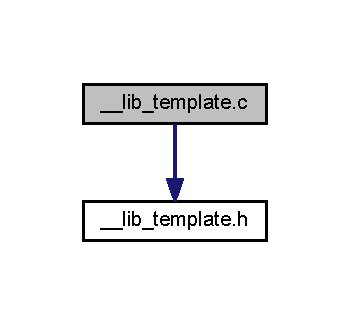
\includegraphics[width=168pt]{____lib__template_8c__incl}
\end{center}
\end{figure}
\subsection*{Macros}
\begin{DoxyCompactItemize}
\item 
\#define {\bf \-\_\-\-\_\-\-M\-O\-D\-U\-L\-E\-\_\-\-H\-E\-A\-D\-E\-R\-\_\-\-\_\-}
\begin{DoxyCompactList}\small\item\em This section was added for the Module Header to be shown on the documentation. \end{DoxyCompactList}\item 
\#define {\bf K8\-\_\-\-C\-O\-N\-S\-T\-A\-N\-T\-S}~3\-U\-C
\begin{DoxyCompactList}\small\item\em Constants (Local or Global) \end{DoxyCompactList}\end{DoxyCompactItemize}
\subsection*{Functions}
\begin{DoxyCompactItemize}
\item 
void {\bf call\-Public\-Functions} ()
\begin{DoxyCompactList}\small\item\em Public Functions are functions that are accessible outside the module. \end{DoxyCompactList}\item 
uint8\-\_\-t {\bf show\-Formula} (uint8\-\_\-t ui8\-X\-\_\-\-Value)
\begin{DoxyCompactList}\small\item\em Formula can also be documented by enclosing it between \textbackslash{}f\$ symbol. \end{DoxyCompactList}\item 
void {\bf main} (void)
\begin{DoxyCompactList}\small\item\em Contains a brief description of what a function does. This brief description can span multiple lines and is terminated by an empty line. \end{DoxyCompactList}\end{DoxyCompactItemize}


\subsection{Macro Definition Documentation}
\index{\-\_\-\-\_\-lib\-\_\-template.\-c@{\-\_\-\-\_\-lib\-\_\-template.\-c}!\-\_\-\-\_\-\-M\-O\-D\-U\-L\-E\-\_\-\-H\-E\-A\-D\-E\-R\-\_\-\-\_\-@{\-\_\-\-\_\-\-M\-O\-D\-U\-L\-E\-\_\-\-H\-E\-A\-D\-E\-R\-\_\-\-\_\-}}
\index{\-\_\-\-\_\-\-M\-O\-D\-U\-L\-E\-\_\-\-H\-E\-A\-D\-E\-R\-\_\-\-\_\-@{\-\_\-\-\_\-\-M\-O\-D\-U\-L\-E\-\_\-\-H\-E\-A\-D\-E\-R\-\_\-\-\_\-}!__lib_template.c@{\-\_\-\-\_\-lib\-\_\-template.\-c}}
\subsubsection[{\-\_\-\-\_\-\-M\-O\-D\-U\-L\-E\-\_\-\-H\-E\-A\-D\-E\-R\-\_\-\-\_\-}]{\setlength{\rightskip}{0pt plus 5cm}\#define \-\_\-\-\_\-\-M\-O\-D\-U\-L\-E\-\_\-\-H\-E\-A\-D\-E\-R\-\_\-\-\_\-}\label{____lib__template_8c_af75326f3ca42905e32d07f10c31e78fb}


This section was added for the Module Header to be shown on the documentation. 

\subsection*{Phil\-Robotics $|$ Philippine Electronics and Robotics Enthusiasts Club}

{\tt http\-://philrobotics.\-com} $|$ {\tt http\-://philrobotics.\-com/forum} $|$ {\tt http\-://facebook.\-com/philrobotics} {\tt phirobotics.\-core@philrobotics.\-com} 

 \begin{TabularC}{2}
\hline
\rowcolor{lightgray}{\bf Filename\-: }&{\bf \char`\"{}\-\_\-\-\_\-lib\-\_\-template.\-c\char`\"{} }\\\cline{1-2}
Description\-: &This is a coding standard template file \\\cline{1-2}
Revision\-: &v00.\-00.\-01 \\\cline{1-2}
Author\-: &Efren S. Cruzat I\-I \\\cline{1-2}
&\\\cline{1-2}
Dependencies\-:&\\\cline{1-2}
\end{TabularC}


\begin{quotation}
This program is free software\-: you can redistribute it and/or modify it under the terms of the G\-N\-U General Public License as published by the Free Software Foundation, either version 3 of the License, or (at your option) any later version. This program is distributed in the hope that it will be useful, but W\-I\-T\-H\-O\-U\-T A\-N\-Y W\-A\-R\-R\-A\-N\-T\-Y; without even the implied warranty of M\-E\-R\-C\-H\-A\-N\-T\-A\-B\-I\-L\-I\-T\-Y or F\-I\-T\-N\-E\-S\-S F\-O\-R A P\-A\-R\-T\-I\-C\-U\-L\-A\-R P\-U\-R\-P\-O\-S\-E. See the G\-N\-U General Public License for more details. \par
\par
 You should have received a copy of the G\-N\-U General Public License along with this program. If not, see {\tt http\-://www.\-gnu.\-org/licenses/}

\end{quotation}


 \begin{TabularC}{4}
\hline
\rowcolor{lightgray}{\bf F\-W Version }&{\bf Date }&{\bf Author }&{\bf Description }\\\cline{1-4}
v00.\-00.\-01 &20120714 &E\-S\-C\-I\-I &Library Initial Release \\\cline{1-4}
\end{TabularC}


Definition at line 32 of file \-\_\-\-\_\-lib\-\_\-template.\-c.

\index{\-\_\-\-\_\-lib\-\_\-template.\-c@{\-\_\-\-\_\-lib\-\_\-template.\-c}!K8\-\_\-\-C\-O\-N\-S\-T\-A\-N\-T\-S@{K8\-\_\-\-C\-O\-N\-S\-T\-A\-N\-T\-S}}
\index{K8\-\_\-\-C\-O\-N\-S\-T\-A\-N\-T\-S@{K8\-\_\-\-C\-O\-N\-S\-T\-A\-N\-T\-S}!__lib_template.c@{\-\_\-\-\_\-lib\-\_\-template.\-c}}
\subsubsection[{K8\-\_\-\-C\-O\-N\-S\-T\-A\-N\-T\-S}]{\setlength{\rightskip}{0pt plus 5cm}\#define K8\-\_\-\-C\-O\-N\-S\-T\-A\-N\-T\-S~3\-U\-C}\label{____lib__template_8c_a28927887322c9fa75b2aebd172f28e38}


Constants (Local or Global) 


\begin{DoxyItemize}
\item + must have prefixed with \char`\"{}\-K$<$\#of\-\_\-bits$>$\-\_\-\char`\"{}
\begin{DoxyItemize}
\item must be written on all caps
\item value must have explicitly defined type 
\end{DoxyItemize}
\end{DoxyItemize}

Definition at line 38 of file \-\_\-\-\_\-lib\-\_\-template.\-c.



\subsection{Function Documentation}
\index{\-\_\-\-\_\-lib\-\_\-template.\-c@{\-\_\-\-\_\-lib\-\_\-template.\-c}!call\-Public\-Functions@{call\-Public\-Functions}}
\index{call\-Public\-Functions@{call\-Public\-Functions}!__lib_template.c@{\-\_\-\-\_\-lib\-\_\-template.\-c}}
\subsubsection[{call\-Public\-Functions}]{\setlength{\rightskip}{0pt plus 5cm}void call\-Public\-Functions (
\begin{DoxyParamCaption}
{}
\end{DoxyParamCaption}
)}\label{____lib__template_8c_a3a6923995f4e3e60ca42cfd6c1b9849b}


Public Functions are functions that are accessible outside the module. 


\begin{DoxyItemize}
\item function name must follow the format $<$action$>$$<$\-Module$>$$<$\-Parameter$>$
\begin{DoxyItemize}
\item e.\-g. get\-Pin\-Value(\-Pin)
\end{DoxyItemize}
\item A prototype of the function must always be defined at the .h file of that module
\item If a function has no parameter the \char`\"{}void\char`\"{} type is omitted to prevent Hi-\/\-Tech C warnings 
\end{DoxyItemize}$<$ Variables local to a function must have assigned values before it can be used 

Definition at line 69 of file \-\_\-\-\_\-lib\-\_\-template.\-c.

\index{\-\_\-\-\_\-lib\-\_\-template.\-c@{\-\_\-\-\_\-lib\-\_\-template.\-c}!main@{main}}
\index{main@{main}!__lib_template.c@{\-\_\-\-\_\-lib\-\_\-template.\-c}}
\subsubsection[{main}]{\setlength{\rightskip}{0pt plus 5cm}void main (
\begin{DoxyParamCaption}
\item[{void}]{}
\end{DoxyParamCaption}
)}\label{____lib__template_8c_a6288eba0f8e8ad3ab1544ad731eb7667}


Contains a brief description of what a function does. This brief description can span multiple lines and is terminated by an empty line. 

Detailed Description can start after the empty line. Entries entered on the detailed description are not shown on the summary view 

Definition at line 99 of file \-\_\-\-\_\-lib\-\_\-template.\-c.

\index{\-\_\-\-\_\-lib\-\_\-template.\-c@{\-\_\-\-\_\-lib\-\_\-template.\-c}!show\-Formula@{show\-Formula}}
\index{show\-Formula@{show\-Formula}!__lib_template.c@{\-\_\-\-\_\-lib\-\_\-template.\-c}}
\subsubsection[{show\-Formula}]{\setlength{\rightskip}{0pt plus 5cm}uint8\-\_\-t show\-Formula (
\begin{DoxyParamCaption}
\item[{uint8\-\_\-t}]{ui8\-X\-\_\-\-Value}
\end{DoxyParamCaption}
)}\label{____lib__template_8c_a3fef8284d54c3b0fb13d2f0dc5196821}


Formula can also be documented by enclosing it between \textbackslash{}f\$ symbol. 

This example function converts the input X to corresponding Y value... \begin{quotation}
$ Y = 3/4 X + 10 $ \end{quotation}


Definition at line 83 of file \-\_\-\-\_\-lib\-\_\-template.\-c.


\section{\-\_\-\-\_\-lib\-\_\-template.\-h File Reference}
\label{____lib__template_8h}\index{\-\_\-\-\_\-lib\-\_\-template.\-h@{\-\_\-\-\_\-lib\-\_\-template.\-h}}
This graph shows which files directly or indirectly include this file\-:\nopagebreak
\begin{figure}[H]
\begin{center}
\leavevmode
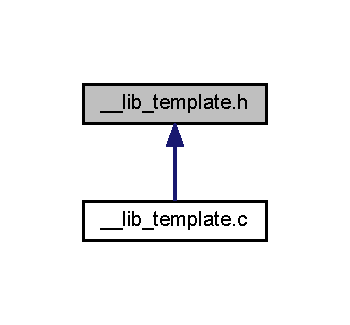
\includegraphics[width=168pt]{____lib__template_8h__dep__incl}
\end{center}
\end{figure}

\printindex
\end{document}
